\relatorio{Estudo e Predição da Exposição de Liquidez de Capital}
    {
        \noindent Pesquisadores: Thiago Hampl, Gabriel Villaça, Giovanna Spirandelli 

        \noindent Projeto de consultoria com DAO Capital
    }
    {O projeto desenvolvido em parceria com o fundo Dao Capital tem como objetivo principal responder à pergunta motivadora: é possível prever a tendência do Ibovespa a partir de indicadores macroeconômicos? Para responder essa pergunta, foi desenvolvido um backtesting robusto que balanceia uma carteira entre índice Ibovespa e a taxa DI (livre de risco). Dessa forma, a simulação da carteira varia a exposição da carteira entre esses dois ativos a partir de diferentes sinais macroeconômicos. Ao fim, não foi possível chegar a um resultado que previa perfeitamente as tendências do Ibovespa, porém houve um cuidado para que o código fosse o mais agnóstico possível, o que significa que não é muito difícil testar outras variáveis e estratégias. 
    }
    {Simulação, Fundo de Investimento, Macroeconomia, Momentum}
    
\section{Introdução}

A equipe de Consultoria 1 do Insper Data trabalhou em conjunto com a gestora Dao Capital a fim de praticar um estudo prático sobre estratégias de variação da exposição de um fundo. A empresa é um fundo quantitativo que utiliza, majoritariamente, estratégias de Momentum na alocação do patrimônio. O orientador do projeto foi o Caio Castro, que auxiliou na execução do projeto em todas as etapas.
O objetivo principal do projeto é pesquisar formas de balancear a exposição de uma carteira genérica a fim de prever momentos de queda e de subida. A equipe não teve acesso à carteira da Dao Capital, a exposição era balanceada entre títulos do Ibov ou taxa livre de risco diária, o DI. Em conversas iniciais com o orientador e outras pesquisas preliminares, uma decisão do grupo foi aplicar a variação de indicadores macroeconômicos como estratégia do projeto, em detrimento de outras opções, como o uso de dados micro empresariais ou técnicos.

A empresa, no entanto, utiliza de prognósticos fundamentalistas para a aplicação de seus métodos quantitativos de gestão. Por isso, não bastava simplesmente desenvolver um código que testa qualquer variável à escolha. Seria necessária uma prova preliminar de que o uso daquela variável para prever o retorno do Ibov era admissível. Por isso, o projeto se dividiu em duas etapas principais, em que a primeira as variáveis eram testadas e uma segunda em as estratégias eram realmente desenvolvidas e, a partir de um backtesting, os resultados de performance da estratégia eram desenvolvidos. 

\section{Regressão}

O teste de variáveis foi feito por um modelo de regressão linear entre o sinal testado e o retorno do Ibovespa, diariamente. Dessa forma, a partir dos resultados da regressão, haveria uma base para afirmar que faz sentido manipular a exposição ao Ibovespa a partir de tal variável. Isso seria justificativa suficiente para que o fundo pudesse aplicar algum possível resultado positivo do projeto na estratégia quantitativa.
Ao final dessa etapa de validação, as variáveis escolhidas para serem usadas na estratégia foram: Índice futuro de commodity, taxa de câmbio dólar real, índice de ações de mercados emergentes, índice S\&P500, juros de longo prazo (5 anos) e futuros de títulos do tesouro dos EUA.

\section{Simulação da Carteira}

As estratégias se resumiram à variação dos sinais macroeconômicos, assim como já descrito. Para calcular a exposição a partir desse sinal, foi utilizado um balanceamento de pesos para calcular a melhor carteira num mesmo período com a mesma variável. Esse peso define o quanto o sinal será relevante para a janela testada, e como unidade de comparação entre carteiras foi utilizado um Sharpe simplificado (retorno da carteira dividido pelo desvio padrão do retorno). 

\begin{equation*}
    Exp = 1 - K \cdot \text{Sinal}
\end{equation*}

Além disso, o cálculo do retorno depende do valor da exposição. Em exposições maiores do que 1, o retorno diário é alavancado em Ibov e perde em DI. Em exposições entre 0 e 1, o retorno é calculado pela soma das duas partes. Já em exposições menores do que 0, o retorno é análogo ao maior do que 1: alavancado em DI e perdendo em Ibov.

No final, o objetivo do projeto é calcular a exposição do próximo dia usando a estratégia numa janela de dias anteriores. Foi definido que a última exposição ideal do backtesting seria a exposição do dia sendo testado e, dessa forma, seria possível calcular uma exposição ideal. Abaixo segue um exemplo prático de cálculo da exposição para um dia:

Utilizando pesos 1, 2, 3 e uma janela de 10 dias, para calcular a exposição ideal do dia 8 de Junho utilizando o índice S\&P500 é calculado as exposições dos últimos 10 dias utilizando os valores da variação do S\&P500 nesses dias com peso 1, peso 2 e peso 3. Com as exposições, é possível calcular o retorno de cada dia utilizando a variação do Ibov nos últimos dias (com shift de 2 dias para simular o atraso de informação). Depois disso, basta calcular o Sharpe entre as 3 séries de performance e escolher a última exposição da série com melhor Sharpe. Com esse método, foi possível calcular a melhor exposição para o dia 8 de Junho para os parâmetros de testes descritos inicialmente. Para um backtesting da carteira utilizando essa estratégia, basta repetir esse método para cada dia da análise e depois calcular a performance a partir das exposições ideiais.

A simulação feita no projeto utilizou uma janela de 180 dias e 30 pesos diferentes (de -3 a 3 com passo de 0.2). Existiam dados de 2007 a 2022 disponíveis para o executar o backtesting. Abaixo segue um exemplo de como os pesos são balanceados para calcular a exposição ideal com os parâmetros descritos acima, utilizando a variação do Câmbio dólar real como estratégia.

\begin{figure}
    \begin{subfigure}{0.45\linewidth}
        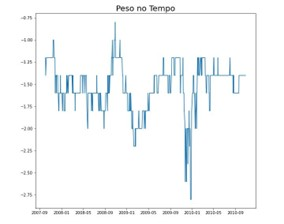
\includegraphics[width = \textwidth]{relatorios/consult/imagens/Imagem1.jpg}
    \end{subfigure}
    \hfill
    \begin{subfigure}{0.45\linewidth}
        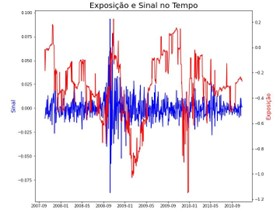
\includegraphics[width = \textwidth]{relatorios/consult/imagens/Imagem2.jpg}
    \end{subfigure}
\end{figure}

\section{Resultados}

Os resultados do backtesting foram separados por período para facilitar o entendimento da performance da carteira em diferentes ciclos econômicos. Abaixo há um exemplo de resultado utilizando a estratégia do indicador de juros a longo prazo:

\begin{figure}[H]
    \centering
    \begin{subfigure}{0.45\linewidth}
        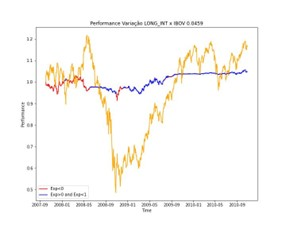
\includegraphics[width = \textwidth]{relatorios/consult/imagens/Imagem3.jpg}
    \end{subfigure}
    \hfill
    \begin{subfigure}{0.45\linewidth}
        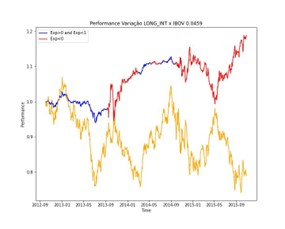
\includegraphics[width = \textwidth]{relatorios/consult/imagens/Imagem4.jpg}
    \end{subfigure}
    \begin{subfigure}{0.45\linewidth}
        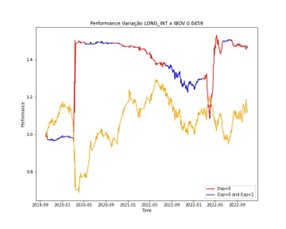
\includegraphics[width = \textwidth]{relatorios/consult/imagens/Imagem5.jpg}
    \end{subfigure}   

\end{figure}

O gráfico de resultado possui duas curvas: a amarela representa a performance do Ibovespa no período, que serve de benchmark para esse projeto. A outra curva representa a performance da carteira variando a exposição a partir da estratégia. Para essa curva, a cor representa o valor da exposição: para exposições menores do que 0, vermelho; entre 0 e 1, azul; maior do que 1, cor verde.

Foram gerados esses 3 gráficos nestes 3 períodos diferentes para todas as 6 variáveis, a fim de entender se a estratégia está realmente conseguindo prever o comportamento do Ibovespa e balanceando a exposição de forma a gerar uma boa performance, entendendo seu comportamento nesses períodos diversos. No entanto, para ter uma resposta plausível sobre a qualidade das estratégias é necessário simular para todo o período, de 2007 a 2022. Abaixo segue a tabela resumo das 6 variáveis, comparando-as com o benchmark.

\begin{figure}
    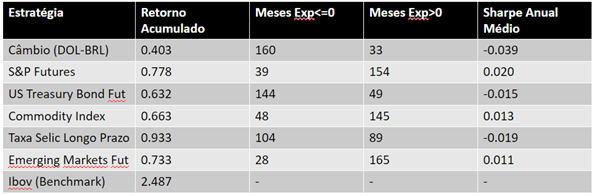
\includegraphics[width = \linewidth]{relatorios/consult/imagens/tabela.png}
\end{figure}

É possível perceber que o retorno acumulado das estratégias não supera o próprio Ibovespa e, por isso, as estratégias não estão conseguindo prever o comportamento do índice. Mesmo que os resultados não sejam positivos, a ferramenta criada para a simulação do backtesting possui código versátil e adaptável, possibilitando pequenas mudanças para testar outras possibilidades de calcular a exposição. 
Uma das possibilidades pensada pela equipe seria adicionar uma informação no cálculo da exposição: a última exposição calculada. Essa informação não é irrealista para o backtesting, já que ao calcular a exposição do dia seguinte, é esperado que a do dia anterior já tenha sido calculada. Com a última exposição, é possível tomar decisões em relação ao cálculo das exposições na janela. Um exemplo seria utilizar dois sinais em uma estratégia, e escolher qual sinal será usado para a janela a partir do valor da última exposição. 

Um exemplo dessa possibilidade de carteira é utilizar o sinal do índice de ações de mercados emergentes para exposições anteriores menores do que 0 e o câmbio dólar real para exposições anteriores maiores que 0. Abaixo segue os resultados dessa estratégia para os períodos estudados anteriormente:

\begin{figure}[H]
    \centering
    \begin{subfigure}{0.45\linewidth}
        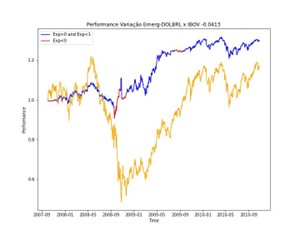
\includegraphics[width = \textwidth]{relatorios/consult/imagens/Imagem6.jpg}
    \end{subfigure}
    \hfill
    \begin{subfigure}{0.45\linewidth}
        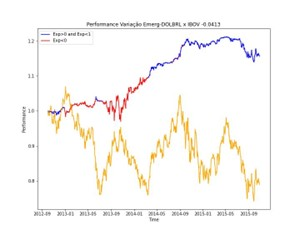
\includegraphics[width = \textwidth]{relatorios/consult/imagens/Imagem7.jpg}
    \end{subfigure}
    \begin{subfigure}{0.45\linewidth}
        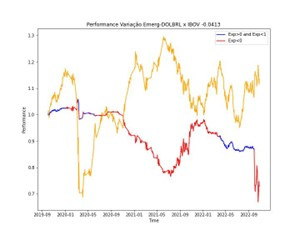
\includegraphics[width = \textwidth]{relatorios/consult/imagens/Imagem8.jpg}
    \end{subfigure}   

\end{figure}

Além disso, foi construído o gráfico também da performance para todo o período de estudo simulando como seria investir nessa carteira a longo prazo.

\begin{figure}
    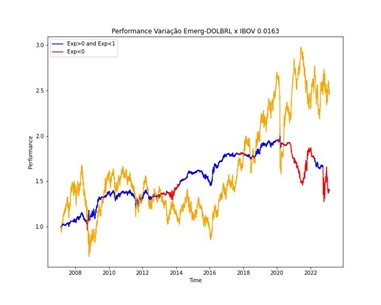
\includegraphics[width = \linewidth]{relatorios/consult/imagens/Imagem9.jpg}
\end{figure}


Para essa estratégia, que muda o sinal da janela dependendo da última exposição calculada, o retorno acumulado foi melhor que qualquer estratégia que utiliza apenas um sinal. 

\section{Conclusão}

Mesmo que o último resultado ainda seja inconsistente e com retorno menor que o próprio Ibovespa, a possibilidade de mudar o código original de forma a testar várias possibilidades de agrupamento de variáveis ou outras estratégias semelhantes evidencia a capacidade da ferramenta desenvolvida. Considerando que o objetivo inicial do projeto era estudar as possibilidades do balanceamento da exposição ao partir de sinais macroeconômicos, é possível concluir que esse estudo foi realizado no escopo definido pela equipe. Além da ferramenta de simulação desenvolvida, ao todo, foram gerados 32 Gráficos do retorno acumulado com mais 13 estratégias diferentes.
